\documentclass[t,aspectratio=169]{beamer}
%\usetheme{Berkeley}
\usepackage{graphicx}
\usepackage{amsmath}
\usepackage[american]{circuitikz}

\title{Clase 12}
\subtitle{Circuitos limitadores, sujetadores y duplicadores}
\author{Dr.-Ing. Juan José Montero Rodríguez}
\subject{Elementos Activos}
\institute{Escuela de Ingeniería Electrónica}
\date{Semestre II-2023}

\begin{document}

\begin{frame}{}
\maketitle
\end{frame}

\section{Recortadores}

\begin{frame}{Aplicaciones de los limitadores (recortadores) de tensión}

\begin{columns}
\begin{column}{0.5\textwidth}

\begin{figure}
    \centering
    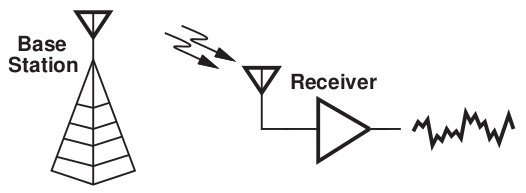
\includegraphics[width=\textwidth]{figures/aplicaciones_limitadores_1.png}
    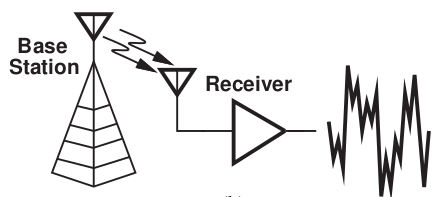
\includegraphics[width=\textwidth]{figures/aplicaciones_limitadores_2.png}
\end{figure}

\end{column}
\begin{column}{0.5\textwidth}

Si un circuito receptor se acerca a la antena de transmisión, la amplitud de la señal recibida aumenta.

\vspace{5mm}Una señal demasiado grande en el receptor podría provocar problemas, como por ejemplo la saturación de los circuitos amplificadores.

\vspace{5mm}En otras ocasiones, un circuito limitador podría proteger ante descargas de arco o picos de sobretensión, si la señal de entrada sobrepasa cierto valor límite.

\end{column}
\end{columns}

\end{frame}

\section{Recortador serie}
\begin{frame}{Recortador serie (diodo ideal)}

\begin{columns}
\begin{column}{0.5\textwidth}

El circuito rectificador de media onda se puede utilizar con cualquier forma de onda de entrada:

\begin{figure}
    \centering
    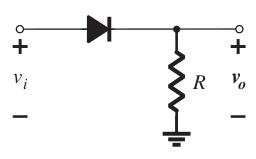
\includegraphics[width=0.5\textwidth]{figures/recortador_serie_ideal_circuito.png}
\end{figure}

La señal se \textbf{recorta} si es \textbf{negativa}, sin importar la forma de onda. 

\vspace{5mm}El circuito deja pasar el resto de la señal sin alterarla.

\end{column}
\begin{column}{0.5\textwidth}

\begin{figure}
    \centering
    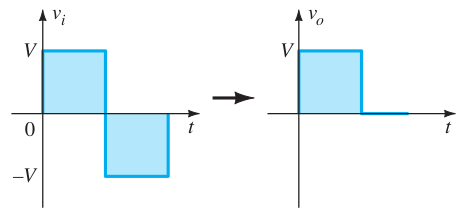
\includegraphics[width=\textwidth]{figures/recortador_serie_ideal_1.png}
    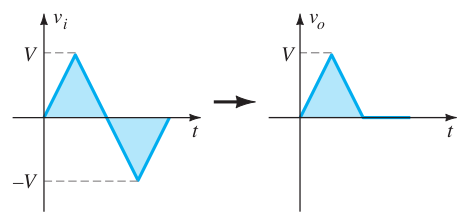
\includegraphics[width=\textwidth]{figures/recortador_serie_ideal_2.png}
\end{figure}

\end{column}
\end{columns}

\end{frame}


\begin{frame}{Recortador serie con fuente CD positiva (diodo ideal)}

\begin{columns}
\begin{column}{0.5\textwidth}

Si se agrega una fuente de CD en serie con el diodo:

\begin{figure}
    \centering
    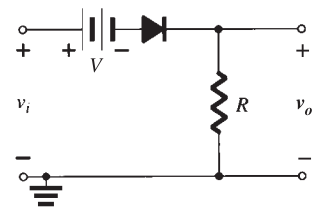
\includegraphics[width=0.5\textwidth]{figures/recortador_serie_ideal_fuente_circuito.png}
\end{figure}

La tensión de la fuente CD se opone a la tensión de entrada, por lo que es necesario aplicar una tensión más alta para lograr la conducción.

\end{column}
\begin{column}{0.5\textwidth}

\begin{figure}
    \flushleft
    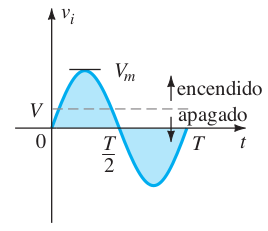
\includegraphics[width=0.5\textwidth]{figures/recortador_serie_ideal_fuente_1.png}
    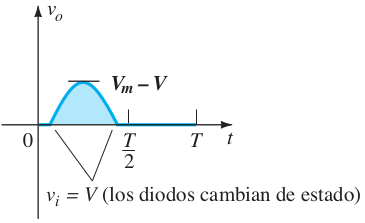
\includegraphics[width=0.65\textwidth]{figures/recortador_serie_ideal_fuente_2.png}
\end{figure}

\end{column}
\end{columns}

\end{frame}


\begin{frame}{Recortador serie con fuente CD negativa (diodo ideal)}

\begin{columns}
\begin{column}{0.5\textwidth}

Si se invierte la polaridad de la fuente de CD:

\begin{figure}
    \centering
    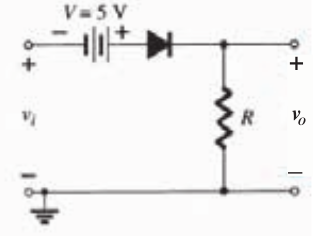
\includegraphics[width=0.5\textwidth]{figures/recortador_serie_ideal_fuente_neg_circuito.png}
\end{figure}

La tensión de la fuente CD contribuye a la tensión de entrada, por lo que es necesario aplicar una tensión más baja para lograr la conducción.

\end{column}
\begin{column}{0.5\textwidth}

\begin{figure}
    \flushleft
    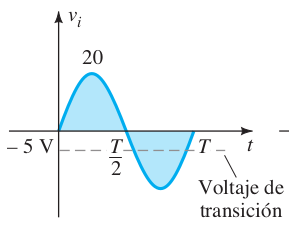
\includegraphics[width=0.5\textwidth]{figures/recortador_serie_ideal_fuente_neg_1.png}
    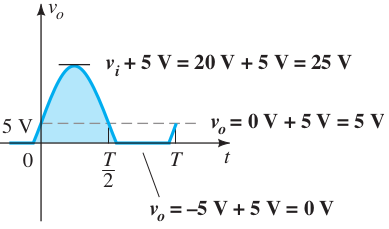
\includegraphics[width=0.65\textwidth]{figures/recortador_serie_ideal_fuente_neg_2.png}
\end{figure}

\end{column}
\end{columns}

\end{frame}


\section{Recortador paralelo}
\begin{frame}{Recortador paralelo (diodo ideal)}

\begin{columns}
\begin{column}{0.5\textwidth}

Si el diodo se conecta en paralelo con la salida, se obtiene un recortador paralelo:

\begin{figure}
    \centering
    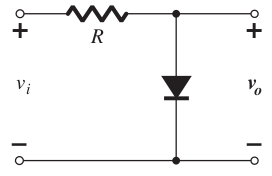
\includegraphics[width=0.5\textwidth]{figures/recortador_paralelo_ideal_circuito.png}
\end{figure}

Este circuito es similar al de un regulador, la diferencia es que aquí se aplica una forma de onda de CA en la entrada.

\begin{itemize}
    \item Si el diodo conduce, la salida es 0.
    \item Si el diodo está abierto, la salida es $v_o = v_i$.
\end{itemize}

\end{column}
\begin{column}{0.5\textwidth}

\begin{figure}
    \centering
    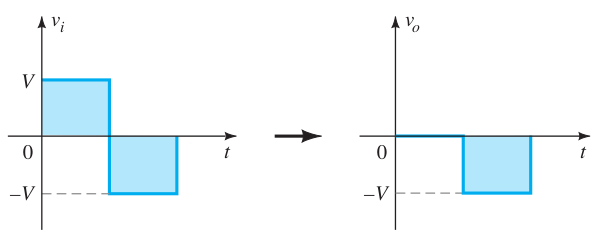
\includegraphics[width=\textwidth]{figures/recortador_paralelo_ideal_1.png}
    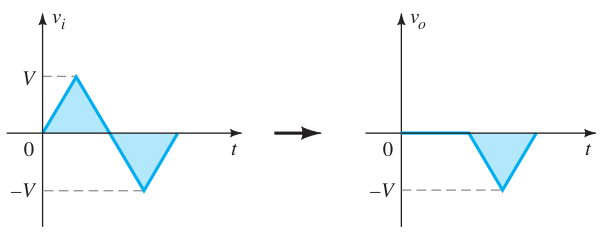
\includegraphics[width=\textwidth]{figures/recortador_paralelo_ideal_2.png}
\end{figure}

\end{column}
\end{columns}

\end{frame}


\begin{frame}{Recortador paralelo con fuente (diodo ideal)}

\begin{columns}
\begin{column}{0.5\textwidth}

Una fuente en serie con el diodo puede contribuir u oponerse a la tensión de la entrada.

\vspace{5mm}Grafique la forma de onda de la tensión de salida si la fuente es de 4 V y la entrada es una onda triangular de 16 Vp.

\begin{figure}
    \centering
    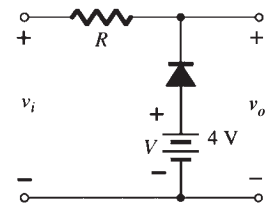
\includegraphics[width=0.5\textwidth]{figures/recortador_paralelo_ideal_fuente_circuito_1.png}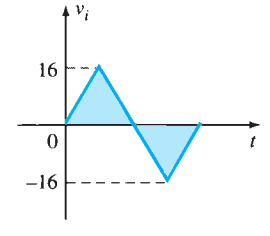
\includegraphics[width=0.5\textwidth]{figures/recortador_paralelo_ideal_fuente_circuito_2.png}
\end{figure}

\end{column}
\begin{column}{0.5\textwidth}

\begin{figure}
    \centering
    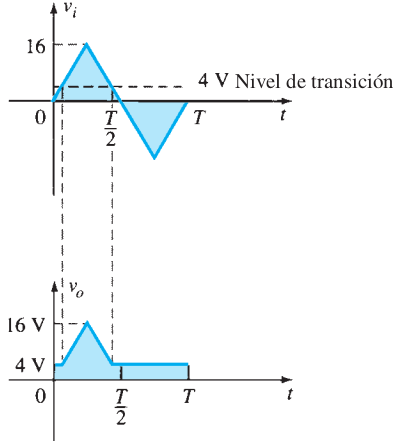
\includegraphics[width=0.8\textwidth]{figures/recortador_paralelo_ideal_fuente_1.png}
\end{figure}

\end{column}
\end{columns}

\end{frame}


\begin{frame}{Recortador paralelo con fuente (diodo de tensión constante)}

\begin{columns}
\begin{column}{0.75\textwidth}

Al incluir un diodo de tensión constante, se debe agregar una fuente de CD de 0.7 V en serie con el diodo, únicamente cuando éste conduce.

\begin{figure}
    \centering
    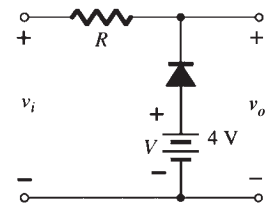
\includegraphics[height=3cm]{figures/recortador_serie_ideal_fuente_vcte_circuito_1.png} \hspace{5mm} 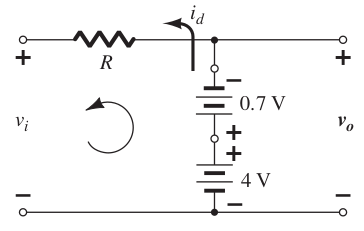
\includegraphics[height=3cm]{figures/recortador_serie_ideal_fuente_vcte_circuito_2.png}
\end{figure}

\end{column}
\begin{column}{0.25\textwidth}

\begin{figure}
    \centering
    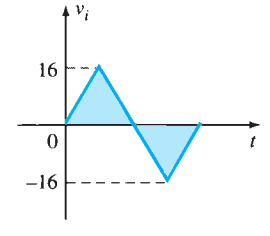
\includegraphics[width=\textwidth]{figures/recortador_serie_ideal_fuente_vcte_1.png}
    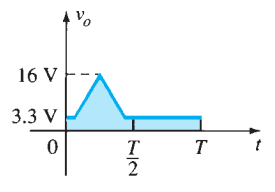
\includegraphics[width=\textwidth]{figures/recortador_serie_ideal_fuente_vcte_2.png}
\end{figure}

\end{column}
\end{columns}

\end{frame}


\section{Resumen}
\begin{frame}{Resumen de recortadores serie}

\begin{figure}
    \centering
    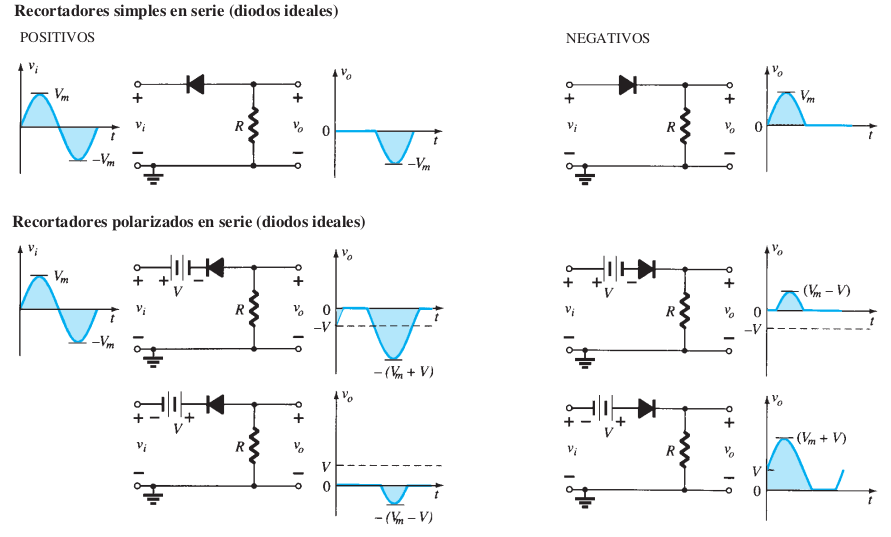
\includegraphics[width=0.8\textwidth]{figures/recortador_serie_resumen.png}
\end{figure}

\end{frame}


\begin{frame}{Resumen de recortadores paralelo}

\begin{figure}
    \centering
    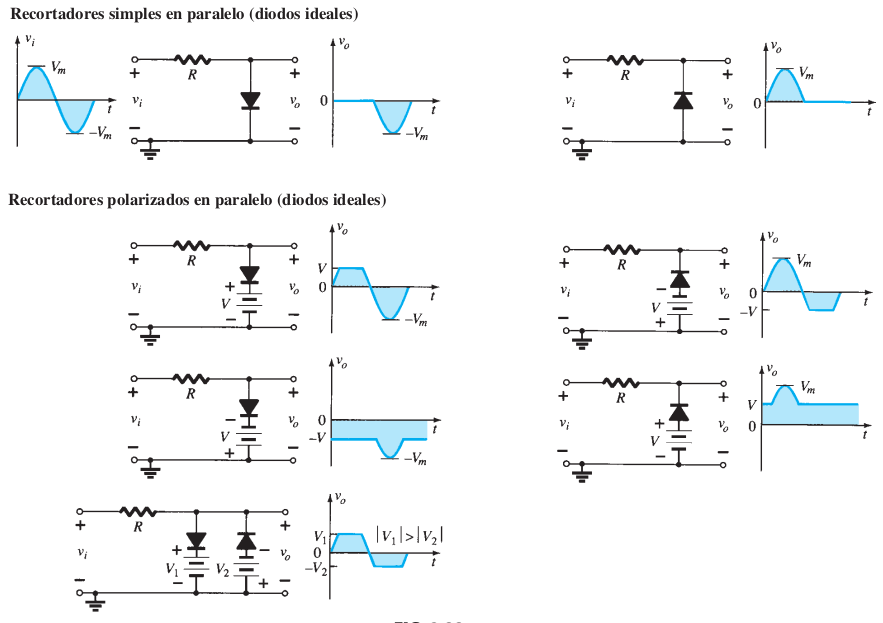
\includegraphics[width=0.7\textwidth]{figures/recortador_paralelo_resumen.png}
\end{figure}

\end{frame}


\section{Funciones de transferencia}
\begin{frame}{Función de transferencia del recortador paralelo (diodo 0.7 V)}

\begin{figure}
    \centering
    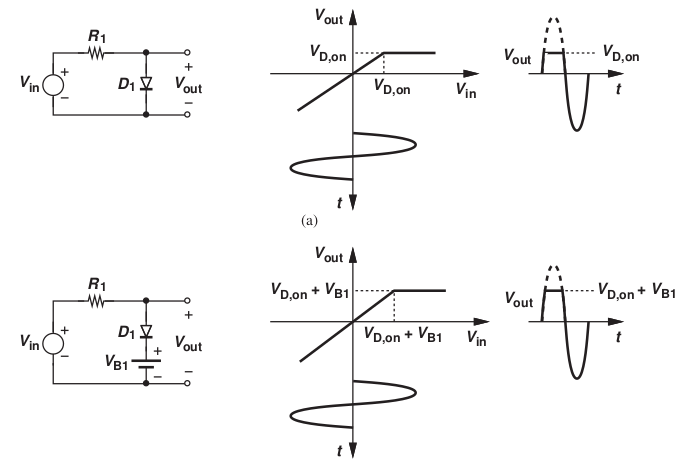
\includegraphics[width=0.7\textwidth]{figures/recortador_paralelo_transferencia_1.png}
\end{figure}

\end{frame}


\begin{frame}{Función de transferencia del recortador paralelo (diodo 0.7 V)}

\begin{figure}
    \centering
    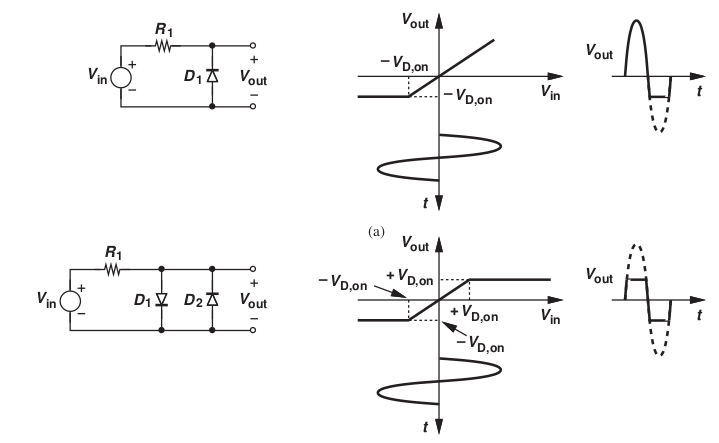
\includegraphics[width=0.7\textwidth]{figures/recortador_paralelo_transferencia_2.png}
\end{figure}

\end{frame}


\begin{frame}{Función de transferencia del recortador paralelo (diodo 0.7 V)}

\begin{figure}
    \centering
    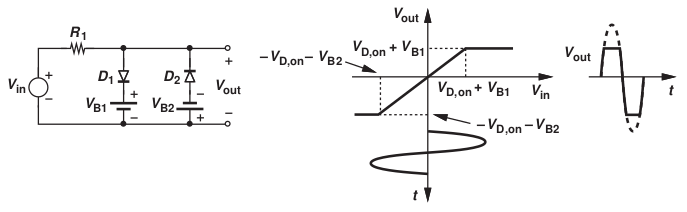
\includegraphics[width=0.7\textwidth]{figures/recortador_paralelo_transferencia_3.png}
\end{figure}

\end{frame}


\section{Ejemplos}
\begin{frame}{Ejemplo 1: Diseño de un limitador de 100 mV}

\begin{figure}
    \centering
    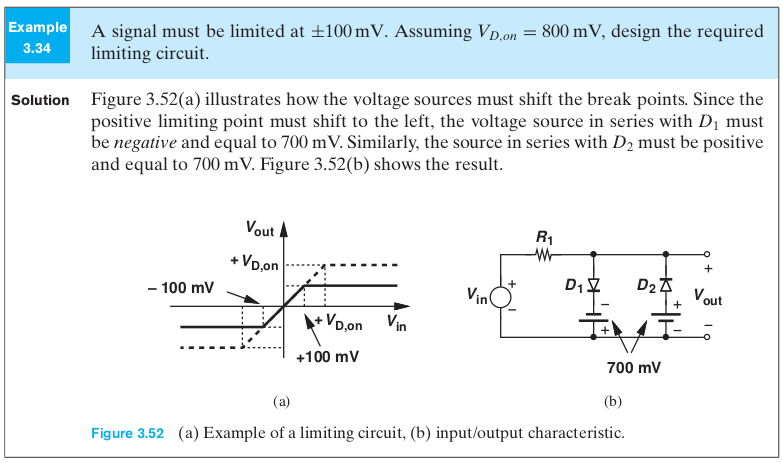
\includegraphics[width=0.8\textwidth]{figures/recortador_ejemplo_1.png}
\end{figure}

\end{frame}


\begin{frame}{Ejemplo 2: Recortadores con formas de onda por secciones}

Considere la función de transferencia mostrada en la figura:

\begin{figure}
    \centering
    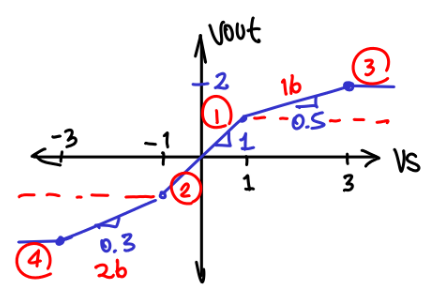
\includegraphics[width=0.5\textwidth]{figures/recortador_ejemplo_2.png}
\end{figure}

Utilizando diodos, resistencias y fuentes de CD, construya un circuito limitador que cumpla con la función de transferencia anterior. Grafique la forma de onda de la tensión de salida si la entrada es una onda triangular de 3 Vp.

\end{frame}


\begin{frame}{Solución 2: Recortadores con formas de onda por secciones}

El circuito que cumple con esta función se muestra a continuación:

\begin{figure}
    \centering
    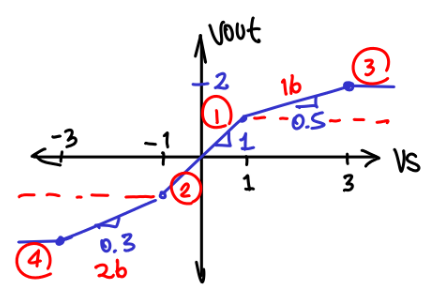
\includegraphics[width=0.45\textwidth]{figures/recortador_ejemplo_2.png}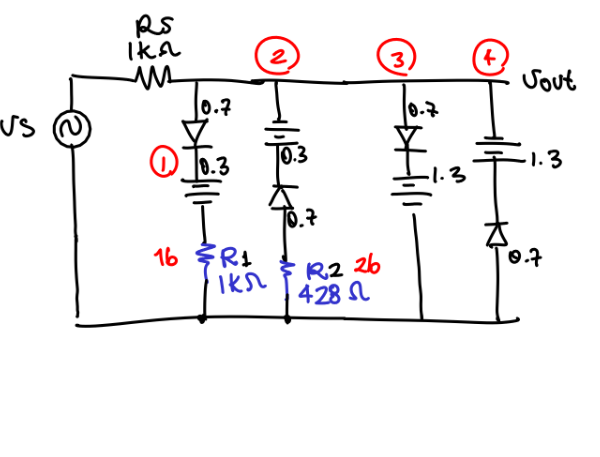
\includegraphics[width=0.55\textwidth]{figures/recortador_solucion_2.png}
\end{figure}

\end{frame}


\begin{frame}{Solución 2: Recortadores con formas de onda por secciones}

El diagrama muestra la forma de onda de la tensión de entrada y la tensión de salida:

\begin{figure}
    \centering
    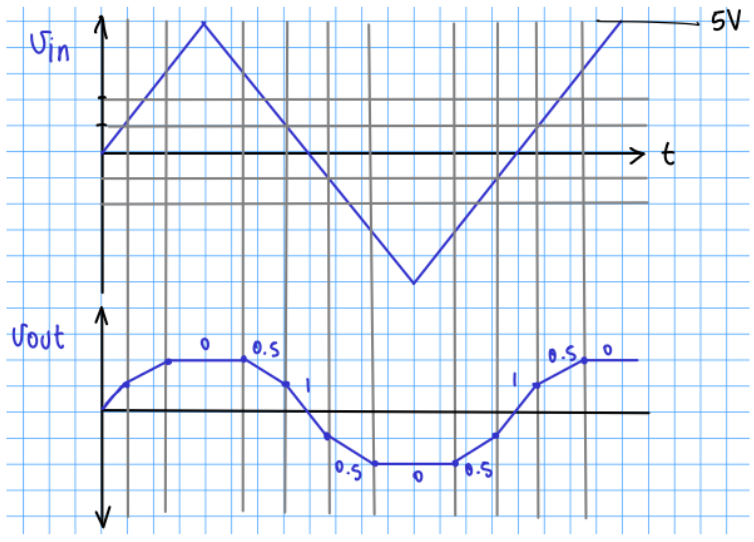
\includegraphics[width=0.6\textwidth]{figures/recortador_solucion_2b.png}
\end{figure}

\end{frame}


\section{Sujetadores}

\begin{frame}{Sujetador de tensión (cambiador de nivel)}

\begin{itemize}
    \item El sujetador de tensión cambia el nivel de CD de una señal, sin alterar la forma de onda.
    \item Se aplica una señal de CA cuadrada, como la que se muestra a la izquierda.
    \item El circuito sujetador contiene un diodo, un condensador y la resistencia de carga.
    \begin{itemize}
        \item Semiciclo positivo: el diodo es un cortocircuito, el condensador se carga.
        \item Semiciclo negativo: el diodo es un circuito abierto, el circuito es RC.
    \end{itemize}
    \item La señal de salida resulta en la señal de entrada desplazada un nivel de CD.
\end{itemize}

\begin{figure}
    \centering
    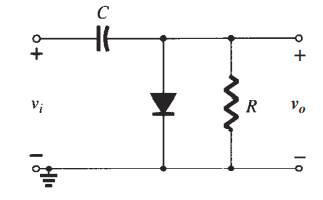
\includegraphics[height=3cm]{figures/sujetador_circuito.png}\hspace{1cm}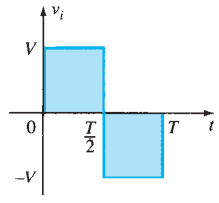
\includegraphics[height=3cm]{figures/sujetador_1.png}\hspace{1cm}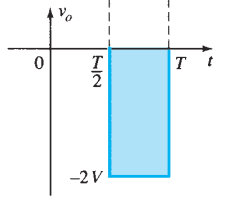
\includegraphics[height=3cm]{figures/sujetador_2.png}
\end{figure}

\end{frame}


\begin{frame}{Análisis del sujetador de tensión}

\begin{columns}
\begin{column}{0.5\textwidth}

\textbf{Semiciclo negativo}

En el semiciclo negativo de $v_{in}$, el diodo está encendido y el condensador se carga hasta $v_c = v_{in}$. La tensión de salida es cero.
%
\[ v_o = 0 \]
%
\centering
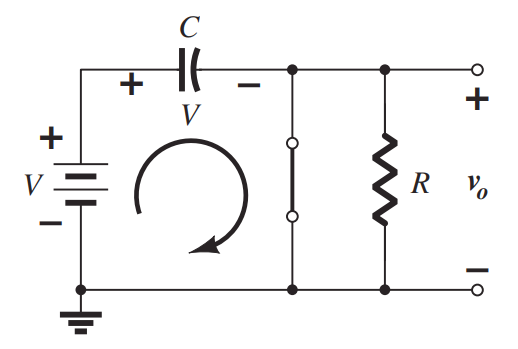
\includegraphics[width=0.7\textwidth]{figures/sujetador_analisis_1.png}

\end{column}
\begin{column}{0.5\textwidth}

\textbf{Semiciclo positivo}

En el semiciclo positivo de $v_{in}$, el diodo está apagado y el condensador se descarga a través de la resistencia. La tensión de salida se encuentra por LVK:
%
\[ v_o = +V_S + V_C = +2V \]
%
\centering
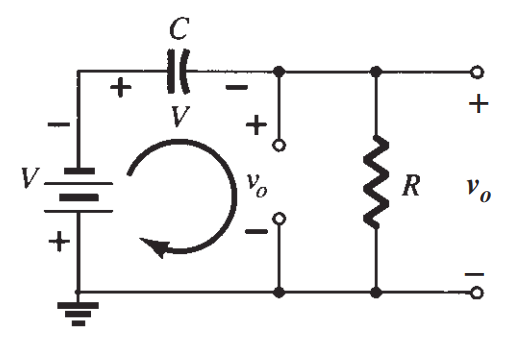
\includegraphics[width=0.7\textwidth]{figures/sujetador_analisis_2.png}

\end{column}
\end{columns}

\end{frame}


\begin{frame}{Cálculo del condensador del sujetador de tensión}

\begin{itemize}
    \item El condensador del sujetador de tensión debe sostener la tensión durante el semiciclo negativo, es decir, durante un tiempo $t = T/2$.
    \item Un circuito RC descarga el condensador completamente en un tiempo $5\tau = 5RC$.
    \item La ecuación de descarga:
    \[ V(t) = V_0 e^{-t/RC} \]
    \item Despejando la capacitancia:
    \[ C = \dfrac{-T/2}{R \ln (V/V_0)} \]
    \item $V/V_0$: porcentaje máximo permitido de descarga
\end{itemize}

\textbf{El condensador se descarga un poco durante el semiciclo negativo, cuando el diodo está abierto. Se vuelve a cargar al máximo en el semiciclo positivo.}

\end{frame}


\begin{frame}{Sujetador con fuente de CD: cambiador de nivel}

Si se agrega una fuente de CD en serie con el diodo, y se aplica una entrada como la que se muestra en la figura:

\begin{columns}
\begin{column}{0.33\textwidth}

    \centering
    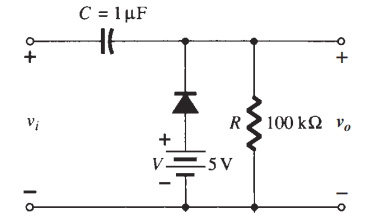
\includegraphics[width=0.8\textwidth]{figures/cambiador_nivel_1a.png}
    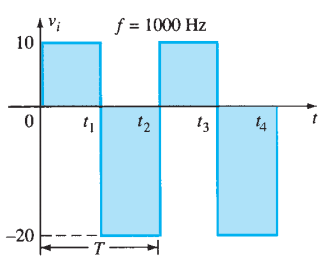
\includegraphics[width=0.8\textwidth]{figures/cambiador_nivel_1b.png}

\end{column}
\begin{column}{0.33\textwidth}

    \textbf{Semiciclo positivo}

    \centering
    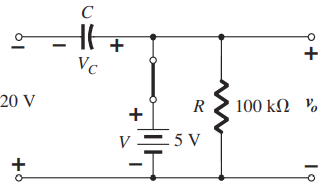
\includegraphics[width=0.8\textwidth]{figures/cambiador_nivel_2.png}

    \flushleft
    \begin{itemize}
        \item El condensador se carga hasta $V_C = 25\ V$.
        \item La tensión de salida es igual a la tensión de la fuente de CD: $V_o = 5\ V$.
    \end{itemize}

\end{column}
\begin{column}{0.33\textwidth}

    \textbf{Semiciclo negativo}

    \centering
    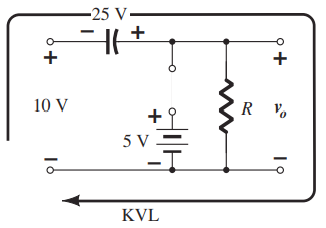
\includegraphics[width=0.8\textwidth]{figures/cambiador_nivel_3.png}

    \flushleft
    \begin{itemize}
        \item La tensión de salida se resuelve por LVK:
        \[ V_o = 10\ V + 25\ V = 35\ V \]
    \end{itemize}

\end{column}
\end{columns}

\end{frame}


\begin{frame}{Sujetador con fuente de CD: cambiador de nivel}

Al analizar el circuito anterior, se observa que el nivel de CD cambia.

\begin{itemize}
    \item La señal de salida ahora es siempre positiva.
    \item El límite inferior de $V_o$ corresponde al valor de la fuente de CD.
\end{itemize}

\begin{figure}
    \centering
    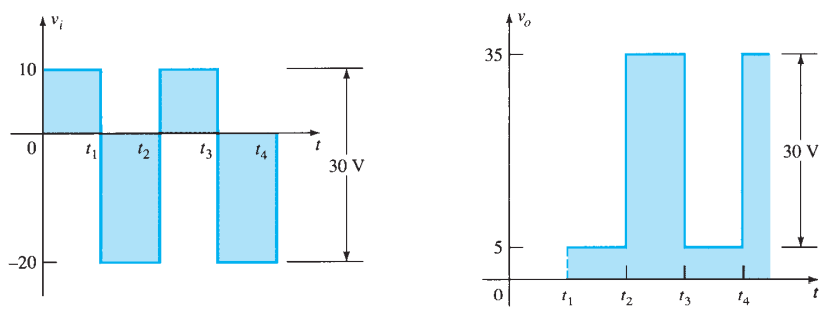
\includegraphics[width=0.7\textwidth]{figures/cambiador_nivel_4.png}
\end{figure}

\textbf{Al ajustar el valor de la fuente de CD en serie con el diodo se puede cambiar el ``offset"}

\end{frame}


\section{Resumen}
\begin{frame}{Resumen de sujetadores}

\begin{figure}
    \centering
    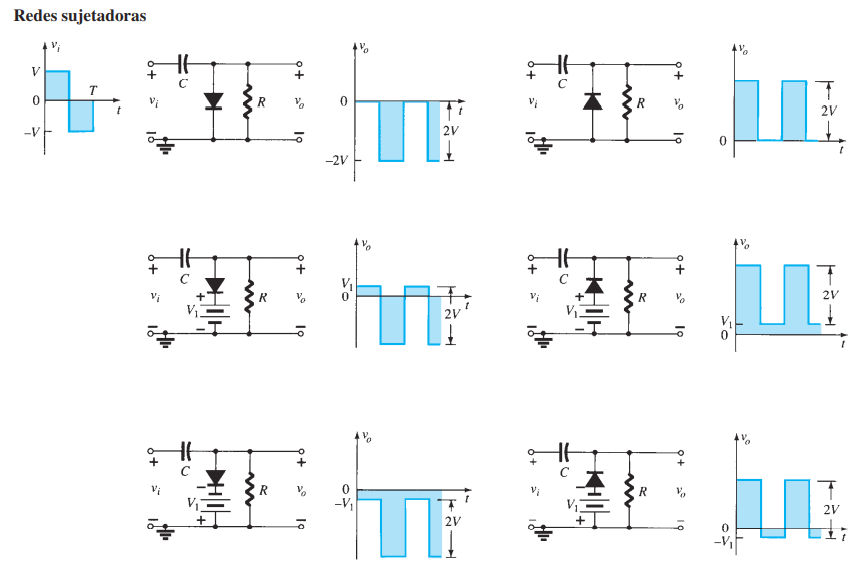
\includegraphics[width=0.8\textwidth]{figures/sujetador_resumen.png}
\end{figure}

\end{frame}


\section{Ejemplos}
\begin{frame}{Ejemplo 3: Sujetador de tensión}

Si la entrada es senoidal, el condensador debe sostener la tensión durante todo T.

\begin{columns}
\begin{column}{0.5\textwidth}

\begin{figure}
    \centering
    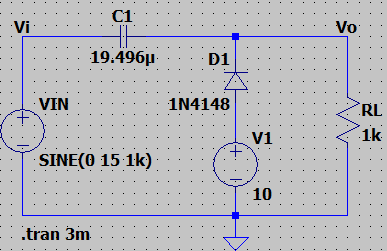
\includegraphics[width=\textwidth]{figures/sujetador_ejemplo_1.png}
\end{figure}
    
\end{column}
\begin{column}{0.5\textwidth}

\begin{figure}
    \centering
    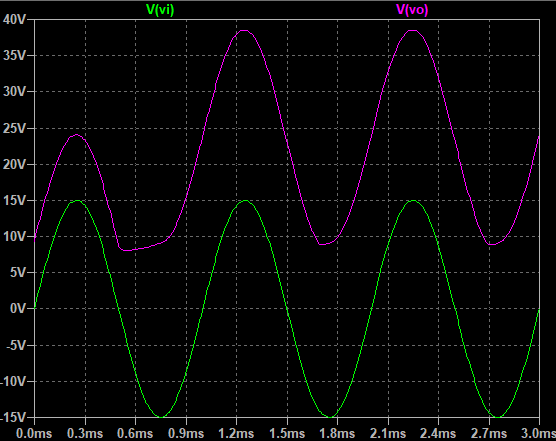
\includegraphics[width=\textwidth]{figures/sujetador_ejemplo_2.png}
\end{figure}

\end{column}    
\end{columns}
    
\end{frame}


\begin{frame}{Ejemplo 3: Sujetador de tensión}

La curva de transferencia se obtiene al cambiar el eje horizontal (tiempo) por la variable de entrada:

\begin{columns}
\begin{column}{0.5\textwidth}

\begin{figure}
    \centering
    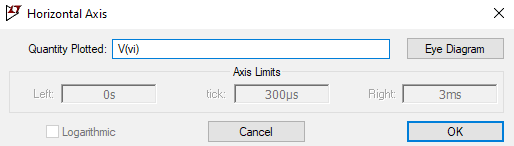
\includegraphics[width=\textwidth]{figures/sujetador_ejemplo_3a.png}
\end{figure}
    
\end{column}
\begin{column}{0.5\textwidth}

\begin{figure}
    \centering
    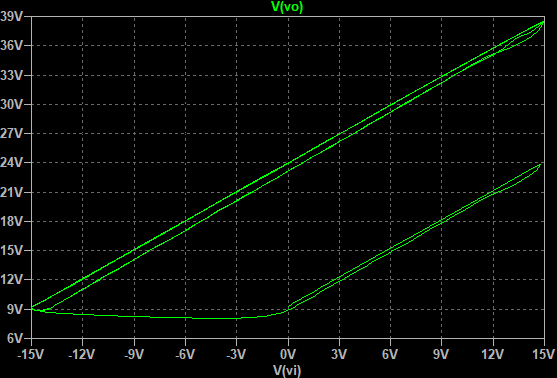
\includegraphics[width=\textwidth]{figures/sujetador_ejemplo_3b.png}
\end{figure}

\end{column}    
\end{columns}
    
\end{frame}


\section{Duplicadores}
\begin{frame}{Duplicador de media onda}

Considere el circuito duplicador de tensión de media onda:

\begin{itemize}
    \item En el semiciclo positivo, D1 en corto, D2 abierto, C1 carga hasta $V_m$.
    \item En el semiciclo negativo, D1 abierto, D2 en corto, C2 carga hasta $2V_m$.
\end{itemize}

\begin{figure}
    \centering
    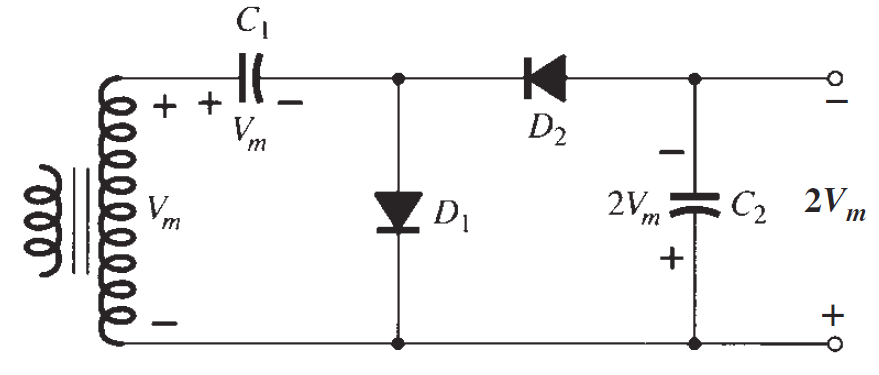
\includegraphics[width=0.7\textwidth]{figures/duplicador_1.png}
\end{figure}

\end{frame}


\begin{frame}{Duplicador de onda completa}

En este circuito se utilizan dos diodos:

\vspace{5mm}
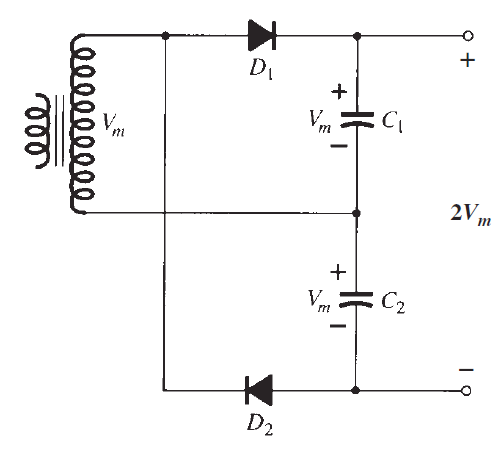
\includegraphics[width=0.4\textwidth]{figures/duplicador_onda_completa_1.png}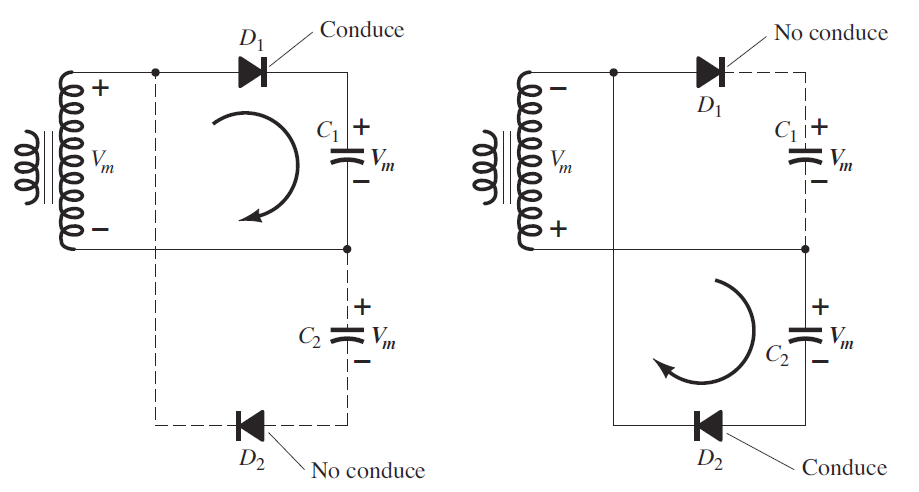
\includegraphics[width=0.6\textwidth]{figures/duplicador_onda_completa_2.png}

\end{frame}


\begin{frame}{Triplicador y cuadriplicador de tensión}

Se permite conectar varias etapas en cascada:

\begin{figure}
    \centering
    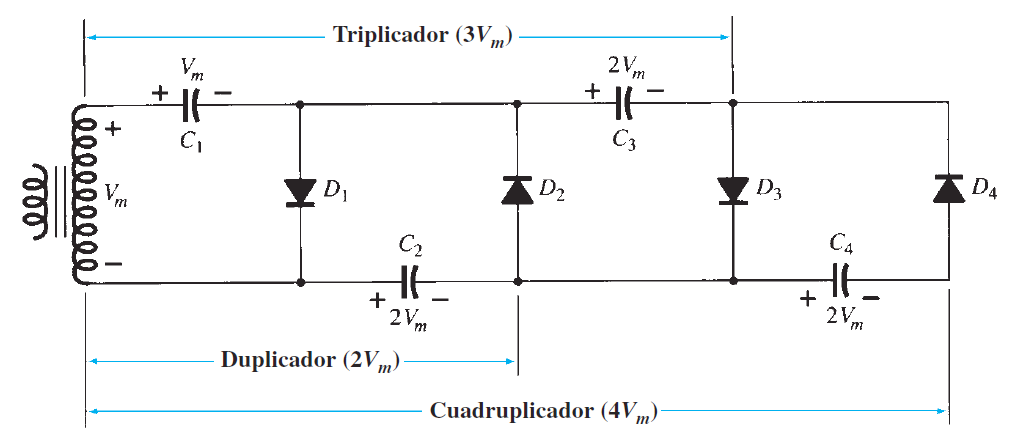
\includegraphics[width=0.7\textwidth]{figures/duplicador_multiples_etapas.png}
\end{figure}

\textbf{¿Se pueden continuar agregando etapas indefinidamente?}

\end{frame}


\begin{frame}{Convertidores CD-CD}

Los convertidores CD-CD permiten cambiar el nivel de CD de una señal:

\begin{figure}
    \centering
    \includegraphics[width=0.4\textwidth]{figures/convertidores_cd_cd_1.png}\hspace{1cm}    \includegraphics[width=0.4\textwidth]{figures/convertidores_cd_cd_2.png}
\end{figure}

Revisar video interesante: \url{https://www.youtube.com/watch?v=H1F4xI2Vgcs}

\end{frame}


\section{Referencias}
\begin{frame}{Lecturas recomendadas}

\begin{itemize}
    \item Boylestad, R. y Nashelsky, L. (2009). Electrónica: Teoría de Circuitos y Dispositivos Electrónicos. Capítulo 2: Aplicaciones de los diodos, pp. 89-92, Pearson Educación, México.
    \item Boylestad, R. y Nashelsky, L. (2009). Electrónica: Teoría de Circuitos y Dispositivos Electrónicos. Capítulo 2: Aplicaciones de los diodos, pp. 101-103, Pearson Educación, México.
    \item Razavi, B. (2013). Fundamentals of microelectronics, 2nd ed., pp. 101-113, Wiley, Los Angeles, California.
\end{itemize}

\end{frame}

\end{document}
